\documentclass[authoryear, 12pt,5p, times]{elsarticle}
%\usepackage[hypcap]{caption}
%\geometry{margin=0.95in,top=1.4in,bottom=1.4in}
\geometry{margin=1.1in,top=1.5in,bottom=1.5in}
\usepackage{float}
\usepackage{amsmath}
\usepackage[hidelinks]{hyperref} 
 \usepackage{gensymb}
\usepackage{subcaption}
\usepackage{url}
%\renewcommand\thefootnote{\fnsymbol{\dagger}}
\usepackage[symbol*]{footmisc}
\makeatletter
\newcommand{\rpm}{\raisebox{.3ex}{$\scriptstyle\pm$}}
\begin{document}
\begin{frontmatter}
\title{Semiconductor Diodes}
\author{\today \quad \\Jung Lin (Doris) Lee [Lab Partner: Leah Tom]\\Prof. William Holzapfel, GSI Thomas Darlington, Thomas Mittiga, John Groh,  \\Victoria Xu, Jonathan Ma, Francisco Monsalve, Xiaofei Zhou\vspace{-30pt}}	 
\end{frontmatter}
\section*{Introduction\label{intro}}
Diodes are isolated pn junctions widely used in everyday electronics such a the common household AC to DC rectifier.
%common ---  electronics  widely used in ----- . Their unidirectional behavior is used for rectification They are used to  convert household AC to DC 
In this lab, we investigated the characteristics of semiconductor diodes. We explored the temperature-dependence of the diode using liquid nitrogen. Using CurveTracer and manually measuring the diode's voltage drop and current , we demonstrate the non-Ohmic VI relation of diodes. We build a diode rectifier and  conduct graphical load line analysis to determine the operating point of the circuit. Finally, we explore different types of diodes, such as light-emitting diode (LED) and the zener diode, their characteristics and applications. 
\section*{3.1}
We connected the 1N4448 diode to the DMM in one direction and measured a resistance of 0.61572$k\Omega$ $\pm$ 0.1138864 $\Omega$. When we reversed direction of the diode and connected the positive grabber to the black band of the diode (Cathode) and the grounding grabber to the red end of the diode(anode), the DMM measured resistance overload. 
\par This shows that diode conducts only unidirectionally, since if there is a non-overloading resistance reading, it means that the tiny test current passed by the DMM actually pass through to the other end of the terminal, resulting in a forward voltage drop across the diode.
\footnote{The minigabbers and BNC cable were connected to the INPUT pairs on the right which had a diode symbol below it.}
\section*{3.2}
In the conducting direction, the plastic-stick mounted 1NN4448 diode has a forward voltage drop of 4.419 mV$\pm$ 4.53$\mu$V.  When we squeezed the diode with our fingers, the measured forward voltage drop is 8.215mV$\pm$ 4.53 $\mu$V. When we submerged the diode in liquid nitrogen, the voltage drop decreased to 2.460mV $\pm$ $4.29\mu V$. The squeezing of the diode with our finger causes slight temperature increase in the diode, which resulted in a lower voltage drop.  We can also see an increasing trend of resistance as we change the temperature of the diode.
\par Diodes do not follow the linear Ohmic behaviour relating voltage and current, but these results still correspond to the semiconductor physics at play. As we decrease the temperature, the conduction electrons has less kinetic energy and therefore slower thermal velocities. Therefore, it requires more work to transport them through the pn junction, since voltage is work per change, the results in a higher voltage drop measured. 
\section*{3.3}
We connect the offset adder to the DMM to measure the output voltage and varied it from -8 to 8 V. Turning the knob clockwise increases the voltage and vice versa for counterclockwise. We loaded up different resistors, since the output current is kept below 24 mA, the circuit is relatively stiff as shown in the slope of in \ref{3_3}. 
\begin{figure}[h!]
\center
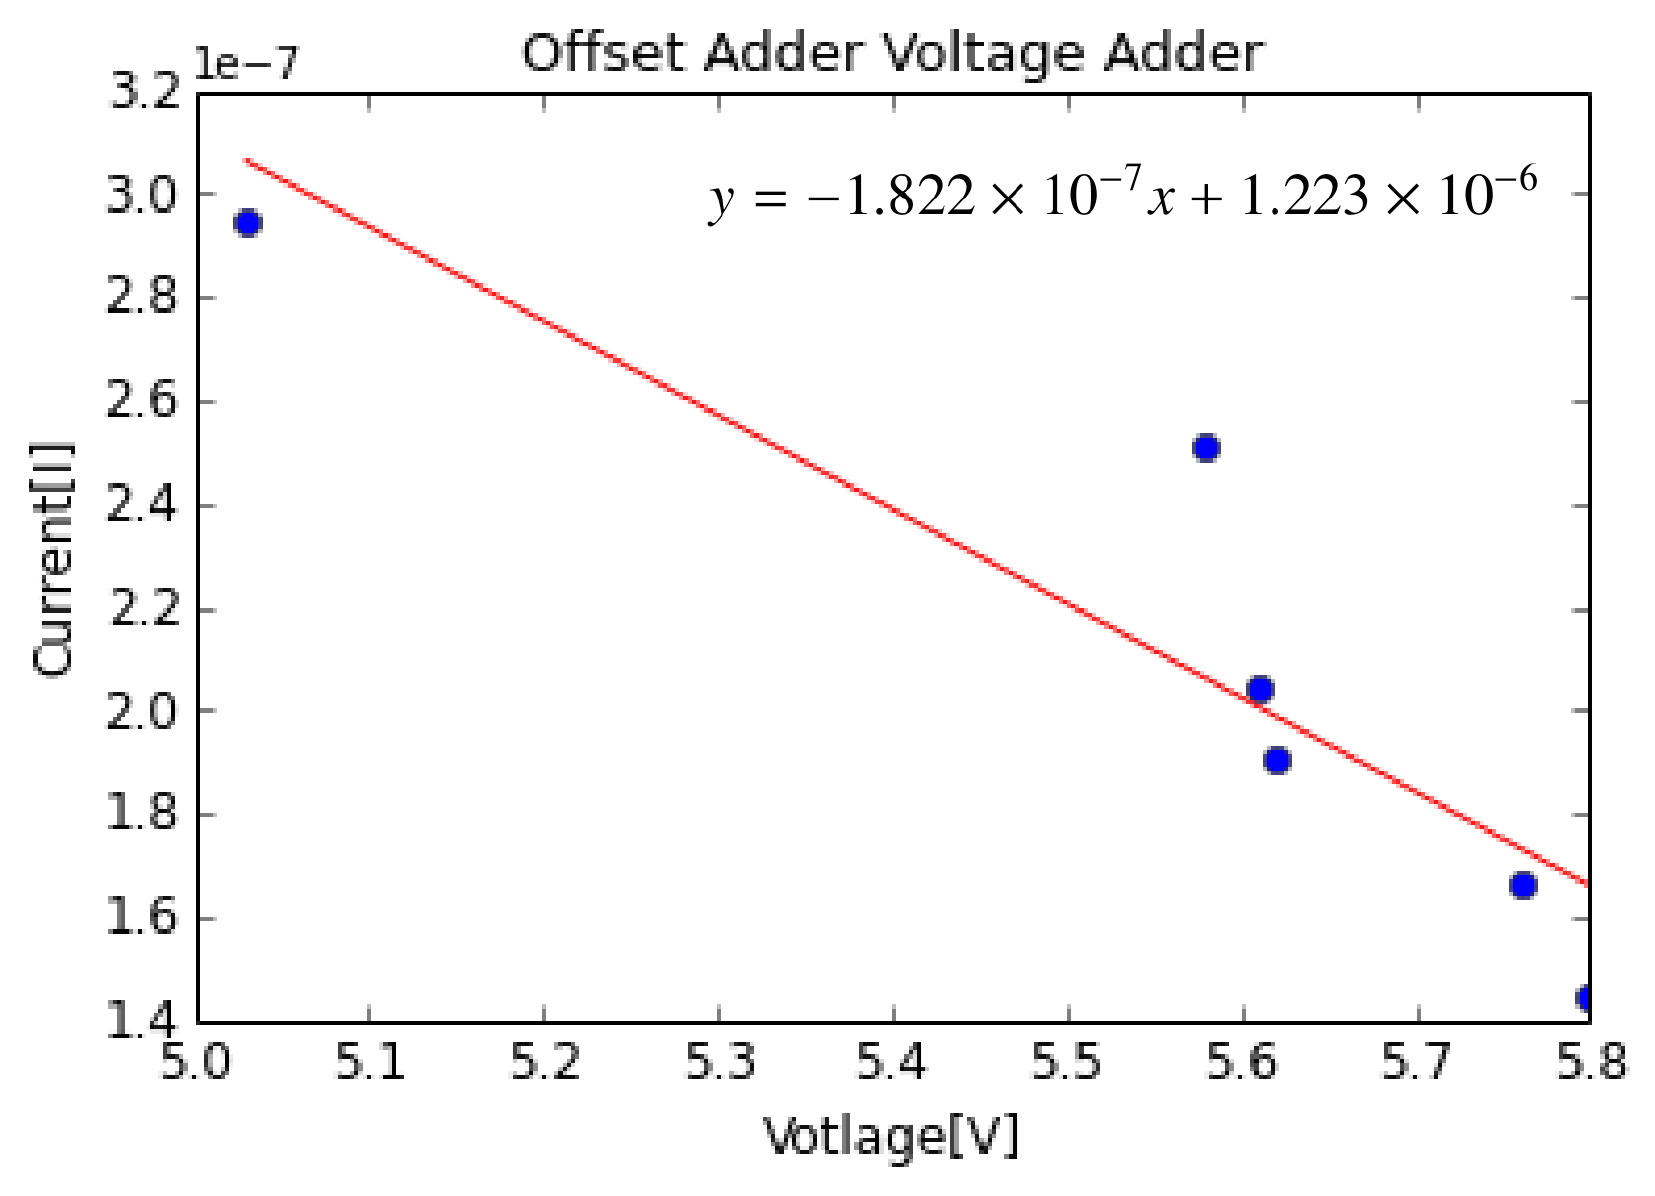
\includegraphics[width=0.5\textwidth]{figure/3_3}
\caption{By plotting the VI curve, since $Z=\frac{\partial V}{\partial I}$, the output  impedance relatively low, at around $-1.822\times10^{-7} \Omega$.}
\label{3_3}
\end{figure}
\section*{3.4}
\begin{figure}[h!]
\center
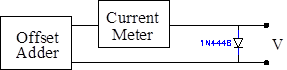
\includegraphics[width=0.3\textwidth]{figure/3_4_diag}
\caption{Setup for measuring the characteristic curve of a diode.}
\label{3_4_diag}
\end{figure}
We setup the circuit as shown in Fig.\ref{3_4_diag}, using the offset adder, we vary the voltage and measure the current using ammeter in series and the voltage across the diode. This manual method used to obtain the characteristic curve yields the plots shown in Fig.\ref{3_4_no_log} and \ref{3_4_log}.
\begin{figure}[h!]
\center
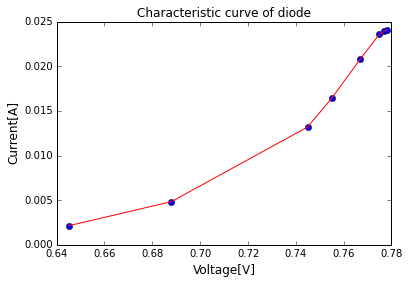
\includegraphics[width=0.5\textwidth]{figure/3_4_no_log}
\caption{The VI curve on a linear scale.}
\label{3_4_no_log}
\end{figure}
\begin{figure}[h!]
\center
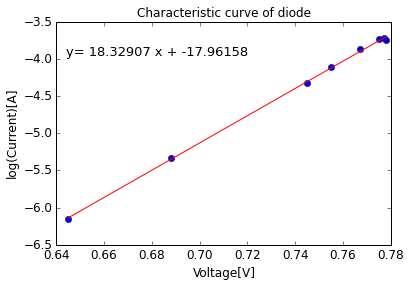
\includegraphics[width=0.5\textwidth]{figure/3_4_log}
\caption{The characteristic curve on with current on a log  scale and voltage on a linear scale.}
\label{3_4_log}
\end{figure}
\section*{3.5}
As shown in Fig.\ref{3_5_norm}, the curve tracer is a more reliable way of finding the characteristic curve of a diode compared to the measurements done in 3.4. This is because the automated adjustment varies the voltage faster to eliminate possible temperature dependent effects due to slow measurement and voltage adjustment.  By selecting the Ohmic (linear) region on the Curve Tracer program, we obtain the $i_{sat}$ and voltage coefficient. 
\begin{figure}[h!]
\center
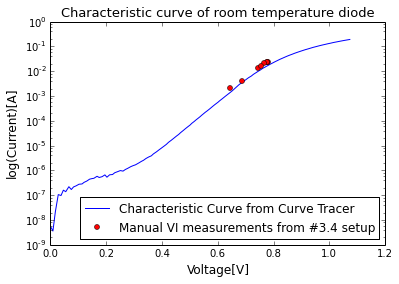
\includegraphics[width=0.5\textwidth]{figure/3_5_norm}
\caption{Characteristic curve for diode at room temperature. (T =298K; $i_{sat}=2.37\times10^{-9}$, voltage coefficient = 16.49) }
\label{3_5_norm}
\end{figure}
\par We rearrange the diode equation as shown in Eq. \ref{diode_eq} and solve for n as in Eq.\ref{n}
\begin{equation}
i(V) = i_{sat}\Bigg[exp(\frac{eV}{nkT})-1\Bigg]
\label{diode_eq}
\end{equation}
\begin{equation}
\begin{split}
n &= \frac{eV}{kT}\frac{1}{ln[\frac{i(V)}{i_{sat}}+1]} \\&= \frac{(1.60\times10^{-19}C)(0.212V)}{1.38\times10^{-23}\frac{m^2kg}{s^{2}K}(298K)}\frac{1}{ln(\frac{6.639\times7A}{2.37\times10^{-9}A}+1)}
\label{n}
\end{split}
\end{equation}
and obtain n= 1.463. Indeed, we do find that the constant n fall within the reasonable range between 1 and 2,  depending on the particular diode. Likewise,% if we evaluate this for a current value of $1.22\times10^{-7}$A and a voltage value of 0.02974V 
for the diode in liquid nitrogen, then we get a n value of 1.427, which is close to the n at room temperature. The n value is characteristic of a diode and should not be significantly affected by the temperature. The characteristic curve of the diode in liquid nitrogen is shown in \ref{3_5_ln2}, where we could see that the Ohmic region on the LN2 curve is shifted rightward compared to the room temperature diode.
\begin{figure}[h!]
\center
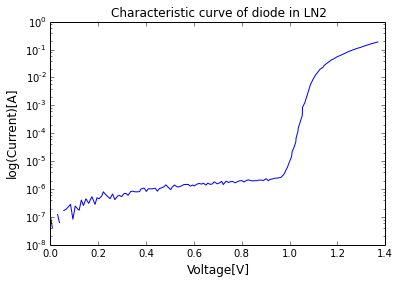
\includegraphics[width=0.5\textwidth]{figure/3_5_ln2}
\caption{Characteristic curve for diode in liquid nitrogen. (T =170K; $i_{sat}=5.22\times10^{-8}$, voltage coefficient =9.59)}
\label{3_5_ln2}
\end{figure}
\section*{3.6}
We setup the experiment by connecting the 1N4448 diode in series with a 1M$\Omega$ resistor and a 12V voltage supply. In order to find the current thoruhg the diode, we measure the value of the voltage drop across the resistor as 327 mV. Using the diode equation (Eq.\ref{diode_eq}), we compute the current through the diode, i(V=327mV), as: 
\begin{equation*}
(4.00\times10^{-8}A)e^{\frac{(1.6\times10^{-19}C)(327\times10^{-3}V)}{(1.4315)(1.38\times10^{-23}m^2kgs^{-2}K^{-1})(298K)}}
\end{equation*}
and obtain current value of 0.2896 mA.
\section*{3.7}\label{3_7_q}
We built a half wave rectifier using the setup shown in Fig.\ref{3_7_setup} and set the DC offset as zero. 
\begin{figure}[h!]
\center
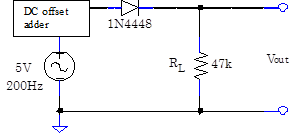
\includegraphics[width=0.5\textwidth]{figure/3_7_setup}
\caption{ setup}
\label{3_7_setup}
\end{figure}
By measuring the input and output signal waveforms, as shown in Fig.\ref{3_7_trace}, we find that the peak-to-peak voltage of the rectified signal is attenuated by a factor of about 8. In addition, we can see that the half-wave rectifier passes half of the signal while blocking the other half, however, there are still some rippling in the rectified signal that requires filtering.
\begin{figure}[h!]
\center
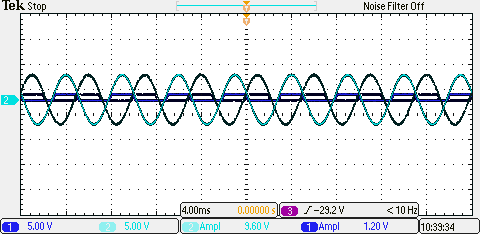
\includegraphics[width=0.5\textwidth]{figure/3_7}
\caption{Scope trace of the AC signal (in cyan; Channel 2) and the rectified output signal (in blue; Channel 1)}
\label{3_7_trace}
\end{figure}
\section*{3.8}
To alleviate the rippling effect observed in Fig.\ref{3_7_trace}, we add a 1$\mu$F capacitor in parallel to the load resistor in the rectifier shown in Fig.\ref{3_7_setup}. The peak-to-peak voltage of the original input signal  is 10V, without the rippling the $V_{pp}$ is equal to the amplitude. With the circuit connected the ripple voltage is at 300mV.
\par a) When we double the input frequency, %the amplitude of the ripple  decreased to 1.25V. %The measured $V_{pp}$ is 1.32V. 
the difference between the $V_{pp}$ and amplitude tells us that the ripple is around 150mV.  This decrease makes sense because the period over which the capacitor discharges remains the same compared to the period of the signal. So over a shorted period, the signal becomes flatter, thus suppressing the ripple amplitude. 
\par  The ripple amplitude decreases as shown in Fig. \ref{ripple}, because we are changing the time constant in the expression $e^{-t/\tau}$. Increase in resistance and capacitance increases the $\tau$, since $\tau$ = RC, causing the signal to flatten and reducing the ripple amplitude. This is proven from the changes to the circuit: 
\par  b) Doubling the capacitance also results in a ripple voltage of around 150mV.
\par c) By doubling the load resistor, the ripple voltage is approximately 150mV.
\begin{figure}[h!]
\center
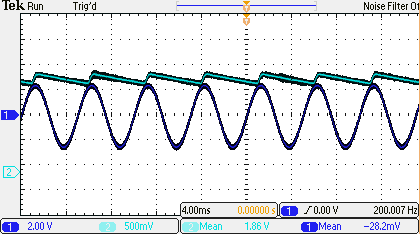
\includegraphics[width=0.5\textwidth]{figure/TEK00015}
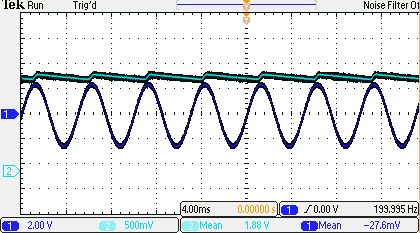
\includegraphics[width=0.5\textwidth]{figure/TEK00017}
\caption{Top: The original waveform. Bottom: The waveform after the rectification, note that the ripple voltage has decreased after the insertion of the load resistor and capacitor.}
\label{ripple}
\end{figure}
\section*{3.9}
We build the circuit as shown in Fig.\ref{3_9_setup} and varied the offset. We measured the output voltage resulting from the different offset as recorded in the table below. We conduct this procedure on both the 1k$\Omega$ and 10k$\Omega$ resistors.
\begin{figure}[h!]
\center
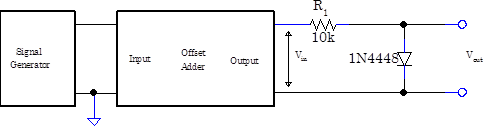
\includegraphics[width=0.5\textwidth]{figure/fig2}
\caption{Circuit setup for 3.9.}
\label{3_9_setup}
\end{figure}
\par We perform the load line analysis using the data we obtained from the experiment as shown in Fig.\ref{ll}. Then we zoomed in on the intersecting regions to find the equilibrium voltage, as demonstrated in Fig.\ref{intersect}. The values are tabulated below for the 1k$\Omega$ and 10k$\Omega$ resistors  in series with the diode.
\begin{figure}[h!]\label{ll}
\center
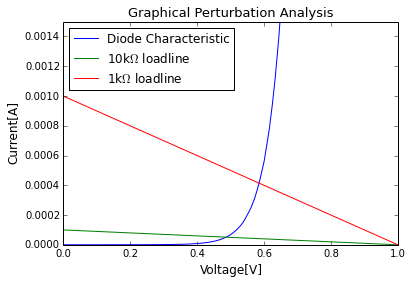
\includegraphics[width=0.5\textwidth]{figure/loadlines}
\caption{Diode characteristic curve and the two load lines corresponding to the different resistors.}
\end{figure}
\begin{figure}[h!]
\center
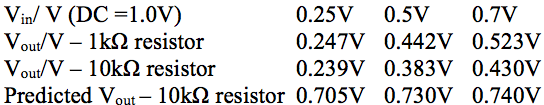
\includegraphics[width=0.5\textwidth]{figure/table}
\label{table}
\end{figure}
The predicted equilibrium point from the load line analysis does not agree with the voltage values that we measured. However, the trend of the data corresponds; both the predicted value and $V_{out}$ measurements shows an increasing trend as expected.
\begin{figure}[h!]
\center
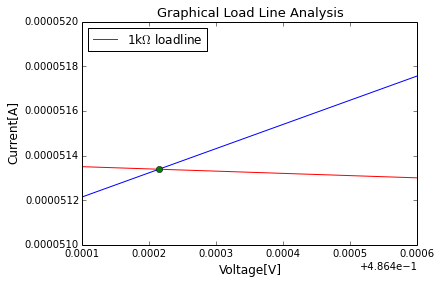
\includegraphics[width=0.5\textwidth]{figure/intersect}
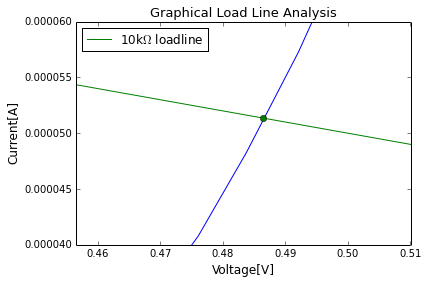
\includegraphics[width=0.5\textwidth]{figure/intersect_10k}
\caption{Top: For the 1k$\Omega$ resistor, the operating point indicated by the intersection occurs at 0.4866V. Bottom: For the 10k$\Omega$ resistor, the operating point indicated by the intersection occurs at 0.4865V.}
\label{intersect}
\end{figure}
\section*{3.10}
For the V$_{pp}$ 2V signal, the offset adder simply adds the input signal with the offset. However, when we vary the amplitude of the input signal to 5V and 10V , we find that the signal have flattened peak. This makes sense because the offset adder limits the maximum V$_{pp}$ of the signal to 2V, therefore, anything signal above 2V gets cutoff and any signal below it is preserved. 
\begin{figure}[h!]
\center
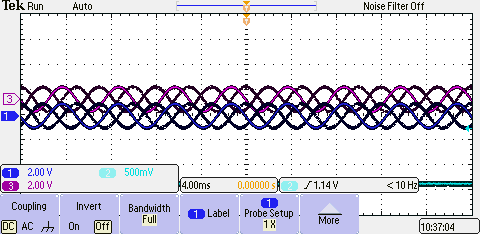
\includegraphics[width=0.5\textwidth]{figure/3_10_12}
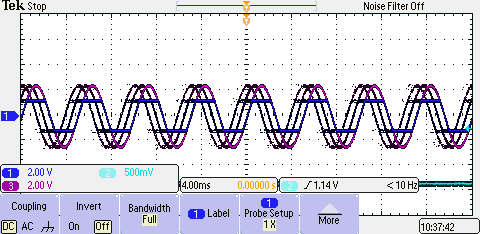
\includegraphics[width=0.5\textwidth]{figure/3_10_13}
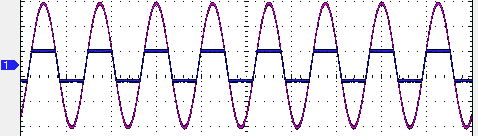
\includegraphics[width=0.5\textwidth]{figure/3_10_14}
\caption{Cropped scope trace showing the original and output signal resulting from varying the amplitude of the signal. (Top figure: 2V ; Middle: 5V; Bottom: 10V). The channel 1 shows the original signal connected directly to the signal generator and the channel 3 shows the output resulting from the offset adder.The y axes is 2.00V per div; the x axes is 4.00ms per div.}
\label{3_10_12}
\end{figure}
%This is shown to be true when we vary the offset adder 
\par A negative offset is applied to a 2 V$_{pp}$ signal, as shown in the upper trace in Fig. \ref{plus_neg}, the signals cuts off and flattens at -1V.  Vice versa for the positive offset, the signal is cuttoff at 1V. In addition to adding an internal offset to the signal, the offset adder also rectifies the signal input and flattens the portion of the signal that exceeds the maximum amplitude cutoff. 
\begin{figure}[h!]
\center
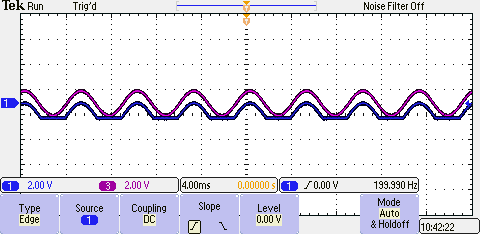
\includegraphics[width=0.5\textwidth]{figure/3_10_17}
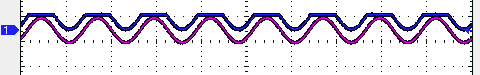
\includegraphics[width=0.5\textwidth]{figure/3_10_16}
\caption{Cropped scope trace showing the original (Ch1) and output (Ch3) signal resulting from varying the amplitude of the signal. (Top figure: Negative Offset ; Middle: Bottom: Positive offset). The y axes is 2.00V per div; the x axes is 4.00ms per div.}
\label{plus_neg}
\end{figure}
The offset adder adds a constant DC component to the input signal. (i.e. it raises the mean of the signal) However, it does not change the amplitude of the signal.
%For 3.10, Pictures 12, 13, 14 (in Dropbox) correspond to the effect of varying amplitude. These correspond to amplitudes of 2V, 5V and 10V respectively. Pictures 17 and 15 to a negative offset and at 2V peak-to-peak. Picture 16 to a positive offset at peak-to-peak amplitude of 2V as well. The offset adder basically cuts off your signal beyond a certain amplitude and offset. 
 
\section*{3.11}
We reconnected the 10k$\Omega$ resistor and diode to the offset adder as shown in  Fig.\ref{3_3}. As shown in the bottom scope trace of Fig. \ref{3_11}, there is equal amplitude of the signal above and below the x axis. The signal does not get rectified like it does in Fig.\ref{3_7_trace} in 3.7.  This makes sense because the offset adder consist of a capacitor inside its circuit. We see an AC signal because the offset adder is a non-zero offset that causes the capacitor to get charged and discharged on each cycle as it alternates. Since the diode is never in reverse bias in this case, the voltage never becomes negative and so the diode allows all the current to pass through. 
\begin{figure}[h!]
\center
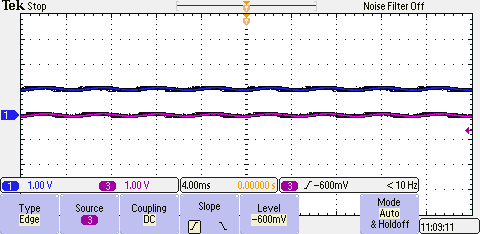
\includegraphics[width=0.5\textwidth]{figure/TEK00022}
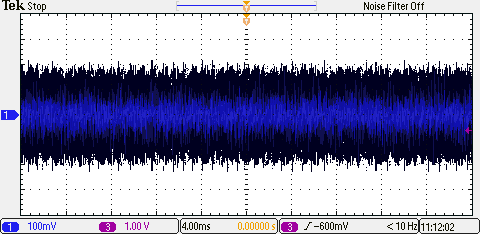
\includegraphics[width=0.5\textwidth]{figure/TEK00024}
\caption{Top: Channel 1 shows the original signal from the signal generator and Channel 3 shows the signal output after passing through the offset adder. Bottom: The scope trace shows the signal behavior after connected to the external Fig.\ref{3_3} circuit.}
\label{3_11}
\end{figure}

\section*{3.12}
As we vary the DC offset, we record the AC component of the output signal, as plotted in Fig.\ref{3_12}. We find that the amplitude of the AC component of the output signal appears to decrease exponentially. When the DC offset is around 0.45V, the amplitude of the signal decays to half of its original amplitude at very low DC offset. 
\begin{figure}[h!]
\center
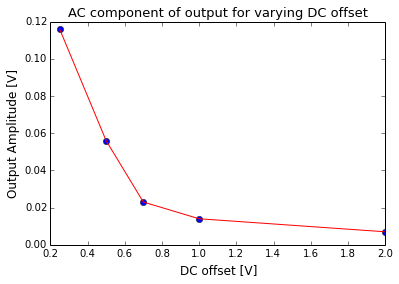
\includegraphics[width=0.5\textwidth]{figure/3_12_fig}
\caption{Exponential decay of AC component of signal as the DC offset is increased.}
\label{3_12}
\end{figure}

\section*{3.13}
When we flipped the polarity of the power supply, the forward voltage drop is close to zero because no current should be flowing through in the reverse direction of a diode. When we connected the LED to different values of resistance, we find that as we increase the resistance, the forward voltage drop increases and the LED brightness dims. When the resistance too large, the voltage drop across the diode is not enough to power the LED since it is below the LED's cutoff voltage, therefore the LED did not light up for the $30k\Omega$ and 300k$\Omega$ trial.
\begin{figure}[h!]
\center
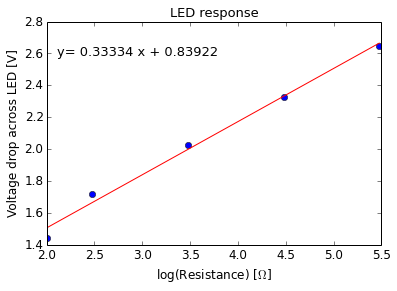
\includegraphics[width=0.5\textwidth]{figure/3_13_LED}
\caption{The LED's brightness decreases as we increase the resistance, corresponding to a larger voltage drop across the resistance.}
\label{3_13_LED}
\end{figure}
\vspace{-20pt}
\section*{3.14}
We used the Curve Tracer to obtain the Fig. \ref{3_14_LED} characteristic curve of the blue LED used in the Problem 3.13. 
\begin{figure}[h!]
\center
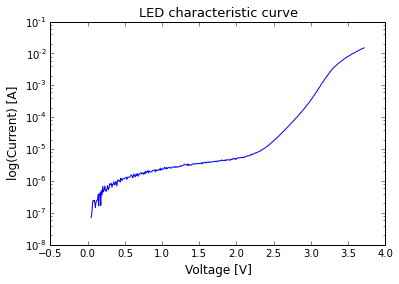
\includegraphics[width=0.5\textwidth]{figure/3_14_LED}
\caption{Characteristic curve of the light-emitting diode (LED). By selecting the Ohmic region of the characteristic curve, the fitting analysis done by Curve Tracer yielded an $i_{sat}$ value of 1.13$\times10^{-9}$A and voltage coefficient of 22.76V.}
\label{3_14_LED}
\end{figure}
\section*{3.15}
The charge stored in a capacitor discharged across a resistor in a RC circuit is described by Eq.\ref{rc}: 
\begin{equation}
Q = Q_0 e^{-t/RC}
\label{rc}
\end{equation}
When the diode is in reverse bias, the alternating current is stopped from flowing in the opposite direction by the diode, and the capacitor discharges into the RC circuit formed with the resistor. Since the capacitor discharges over half a cycle, we are interested in the voltage across the capacitor at that time:
%\begin{align*}
%V(t=\frac{1}{2f}) = \frac{Q_0e^{-1/(2fRC)}}{C} 
%\\
%\end{align*}
\begin{equation}
\begin{split}
V\Big(t=\frac{1}{2f}\Big) &= \frac{Q_0e^{-1/(2fRC)}}{C}  \\&= V_0 e^{-1(2fRC)}
\end{split}
\end{equation} The ripple voltage is the difference between this voltage and $V_0$: 
\begin{equation}
V_{ripple} = V_0(1-e^{-1/(2fRC)})
\end{equation}
For the nominal values in 3.8, C=1$\mu$F and R=47k$\Omega$, $V_0$=5V:
$$V_{ripple} = 5V(1-e^{-1/(2(200Hz)(47k\Omega)(1\mu F))})=259mV$$
This is close to the amplitude of the ripple shown in the original waveform in Fig.\ref{ripple}. \footnote{Estimated as 6/10 of a division, each division is 500mV.}
As we doubled the f,R,or C, in 3.8, the new ripple voltage is 131mV, approximately equal to the corresponding estimate of the ripple voltage (150mV) for the lower figure of Fig.\ref{ripple}.
\section*{3.16}
We performed the graphical perturbation analysis by offsetting our load line by the offset adder value as shown in Fig.\ref{perturb}. We chose these offsets because they are small changes to the system parameters for the perturbation analysis.  We find the intersection between the new load line and the characteristic curve of our diode. Graphically, we observe that the $\Delta V$ is around 0.02, 0.015 and 0.015V which is much smaller than the change in battery voltage $\Delta V_0$ 0.25, 0.50 and 0.75V respectively. The intersecting points for the operating point does not agreee with our reselts. This is because we are assuming a linear change in our perturbation analysis; however, the DC off setter also cuts off the signal beyond the maximum voltage, resulting in the decreasing relation shown in Fig.\ref{3_12}.
\begin{figure}[h!]
\center
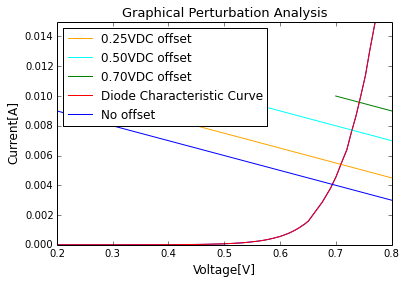
\includegraphics[width=0.5\textwidth]{figure/doris}
\caption{Graphical perturbation analysis of loadlines with different offset values.}
\label{perturb}
\end{figure}
\section*{3.17}
Using the offset load lines in 3.16 and the diode characteristic curve, we computed the slope of the characteristic curve at each computed operating points. The reciprocal of this computed slope yields the small signal impedance at each of these points, since the differential impedance is computed by $Z=\frac{\partial V}{\partial I}$ and the slope is $\frac{\partial I}{\partial V}$.  
\begin{figure}
\center
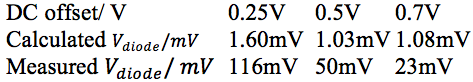
\includegraphics[width=0.5\textwidth]{figure/table1}
\end{figure}
\begin{figure}[h!]
\center
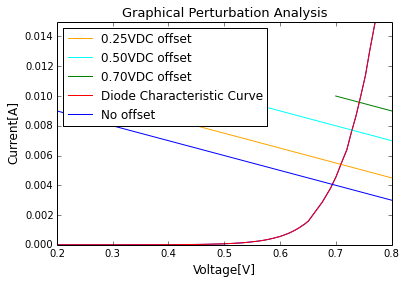
\includegraphics[width=0.5\textwidth]{figure/doris}
\caption{The derivative at the particular point was computed by the finite difference differentiation of $[f(x+h)-f(x)]/h$ where h is a small voltage step. }
\label{slope}
\end{figure}
We assumed that the diode was a resistor in a circuit in series with a 10kΩ resistor and based on the voltage divider equation:
\begin{equation}
V_{diode}=  Z_{diode}/(Z_{diode}+10k\Omega)  V_0
\end{equation}
The values we obtained for voltage across diode using small signal impedance perturbation analysis are compared against the values we measured below.
\begin{figure}
\center
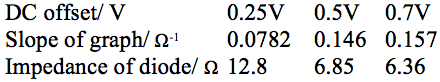
\includegraphics[width=0.5\textwidth]{figure/table2}
\end{figure}
\par  As shown in \ref{bad}, our prediction did not agree with the data from 3.12  but shows the same general decreasing trend. If we used the large-signal impedance instead, it would yield a voltage divider output much larger than the actual answer because the function describing the characteristic curve is monotonically increasing and the slope is also increasing. So if we compute the finite sum differentiation over a large step, then the resulting slope would be larger.
\begin{figure}[h!]
\center
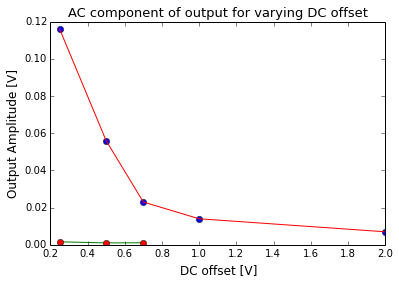
\includegraphics[width=0.5\textwidth]{figure/bad}
\caption{Plotting the predictions on the 3.12 graph. The green line is the prediction and the red line is the data from 3.12.}
\label{bad}
\end{figure}
\section*{3.18}
We designed the zener diode voltage regulator shown in Fig. \ref{3_18_schematic}, as a voltage divider with one resistor and the 1N5234 zener diode. We compute the resistance given that the maximum current can not exceed 15mA:
\begin{equation}
R_s = \frac{V_{in}-V_{out}}{I_{max}}=\frac{12-6.2 V}{15mA} =386.67\Omega
\end{equation}
We construct the necessary $R_s$ by putting a 80,300, and 4$\Omega$ resistor in series. For the 12V$\pm$1.84mV input from the breadboard box, the output voltage regulated by this circuit is measured at 6.2946 V$\pm$1.155 mV.
\begin{figure}[h!]
\center
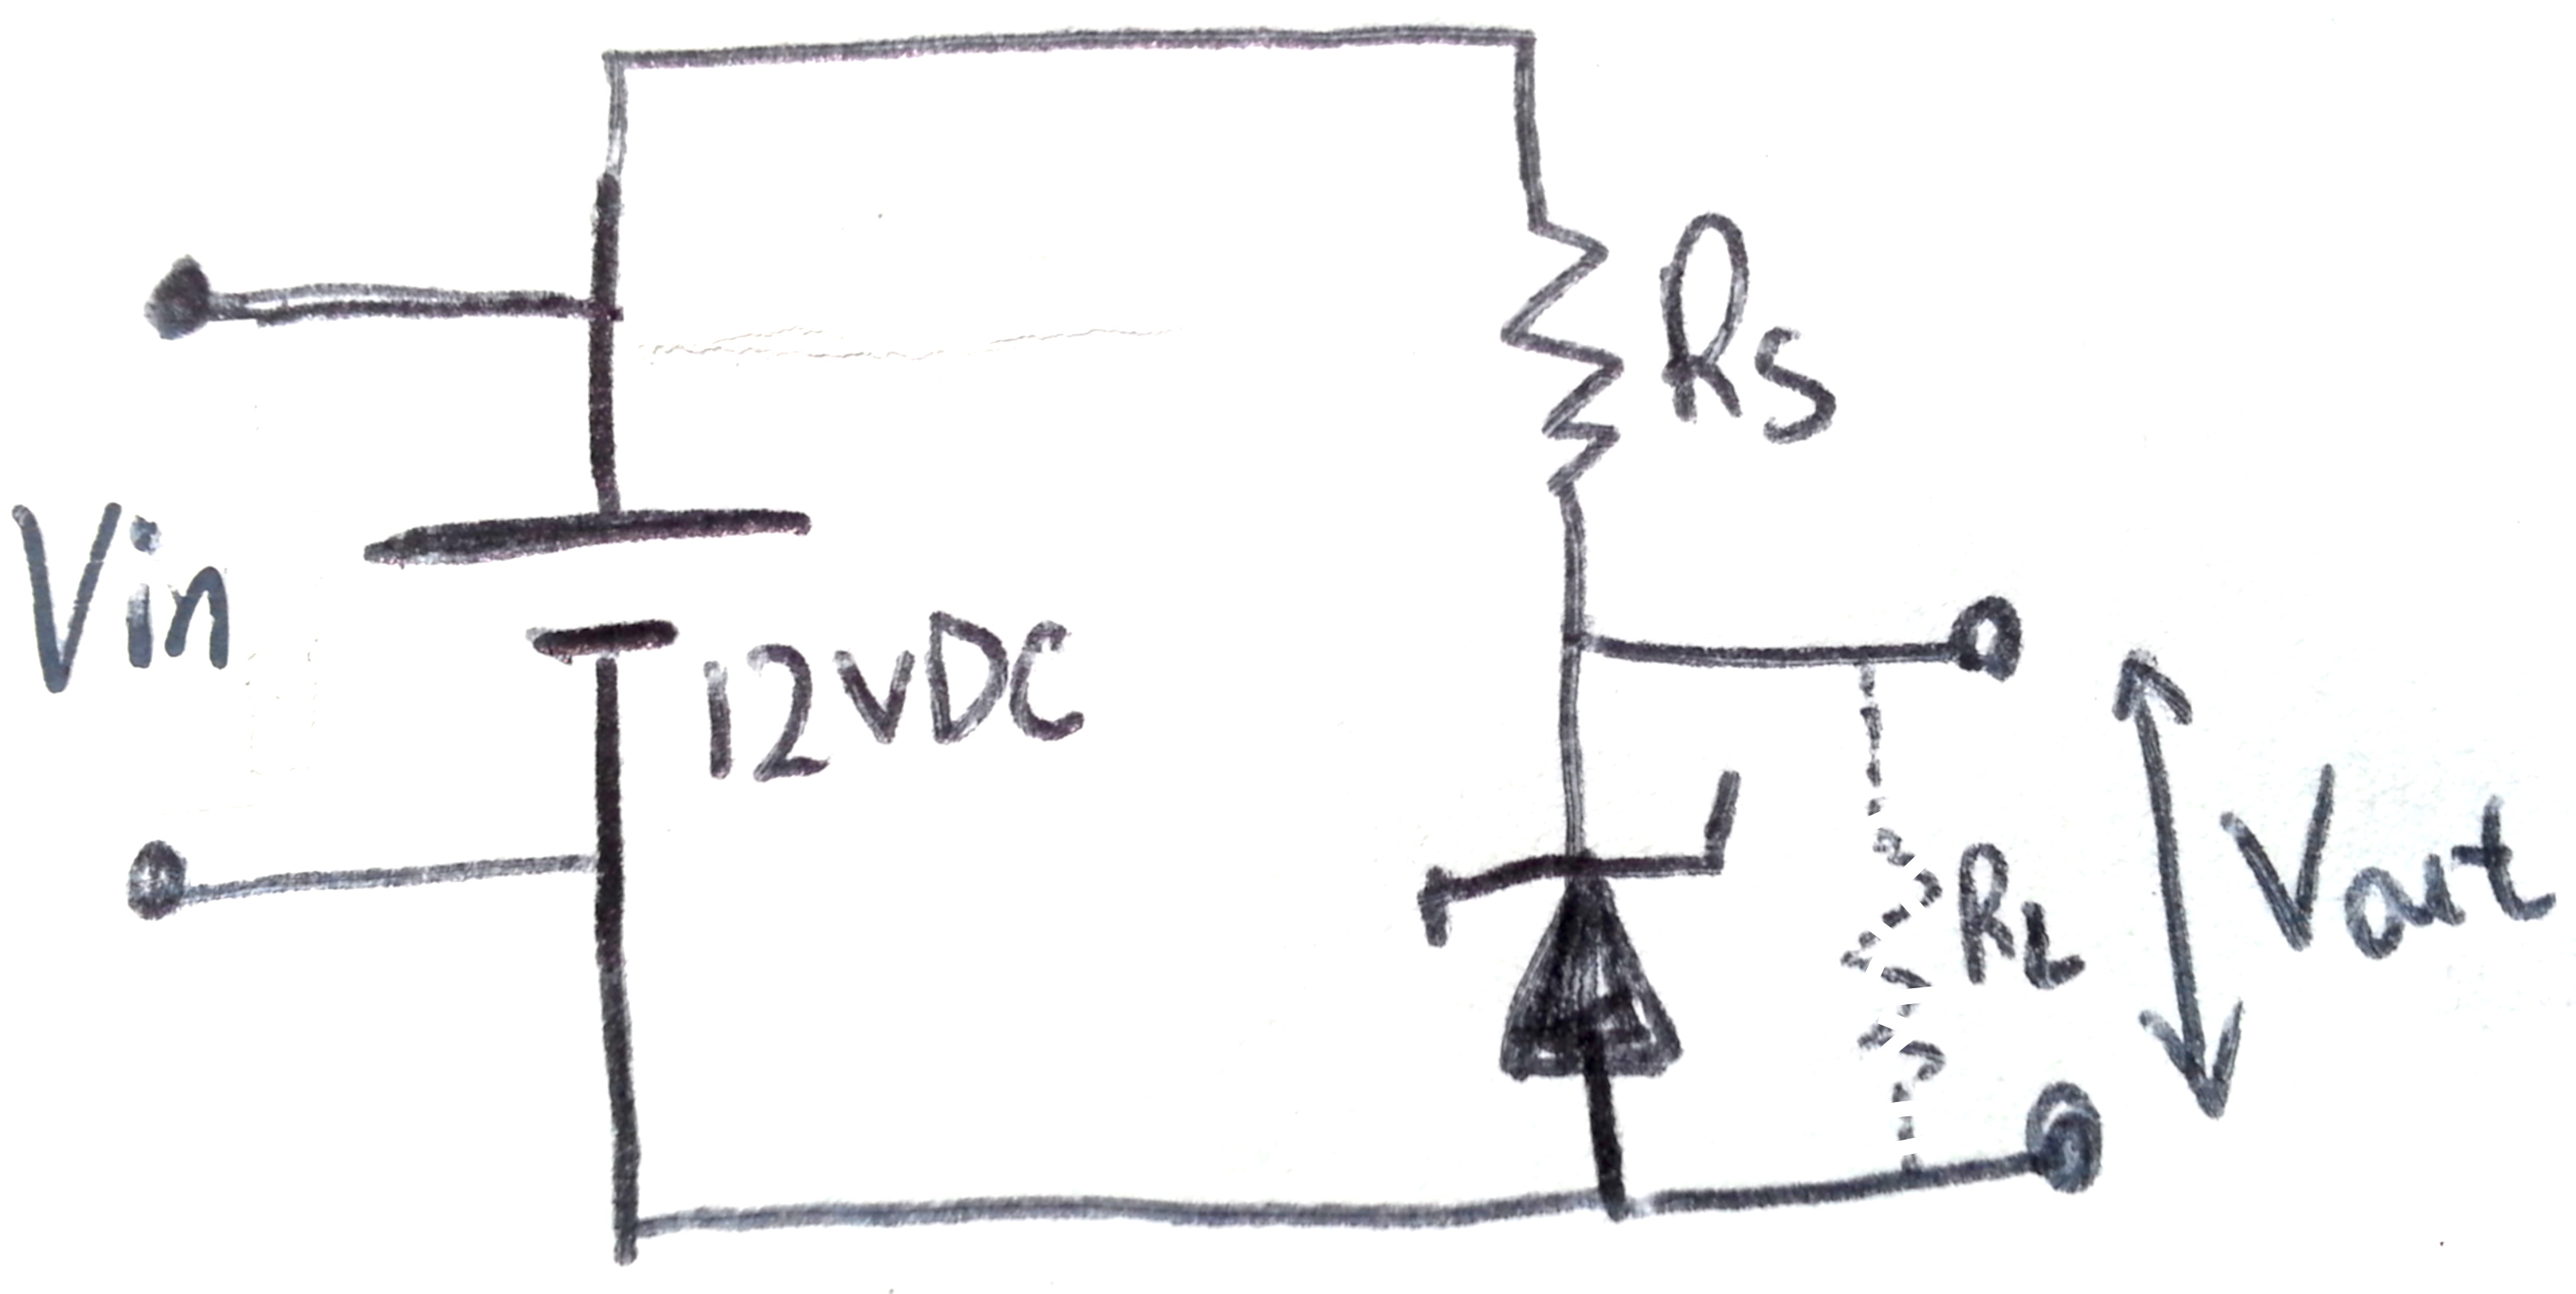
\includegraphics[width=0.5\textwidth]{figure/3_18_schematic}
\caption{Schematic for the zener diode voltage regulator.}
\label{3_18_schematic}
\end{figure}
If we want a less than 5\% decrease in output voltage, then the minimum voltage that satisfies this condition is 5.89V. So the smallest load resistor that will not significantly decrease the circuit output voltage is around 189$\Omega$. 
\begin{figure}[h!]
\center
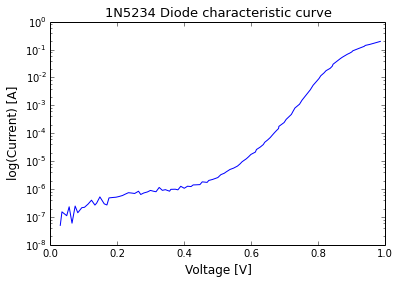
\includegraphics[width=0.5\textwidth]{figure/3_18_curve}
\caption{Characteristic curve of the 1N5234 zener diode. }
\label{3_18_curve}
\end{figure}
\section*{3.19}
\begin{figure}[h!]
\center
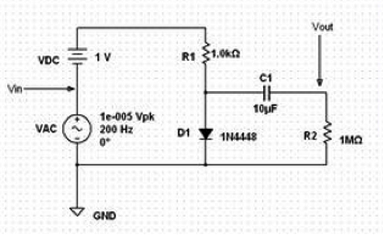
\includegraphics[width=0.5\textwidth]{figure/3_19_setup}
\caption{BiasDiode simulation on MultiSim.}
\label{3_19_setup}
\end{figure}
The BiasDiode simulation setup is shown in Fig.\ref{3_19_setup}. When the signal generator has $V_{pp}$=$1\times10^{-5}$V, the input and output signal is shown in Fig.\ref{firstrow}.
\begin{figure}[h!]
\center
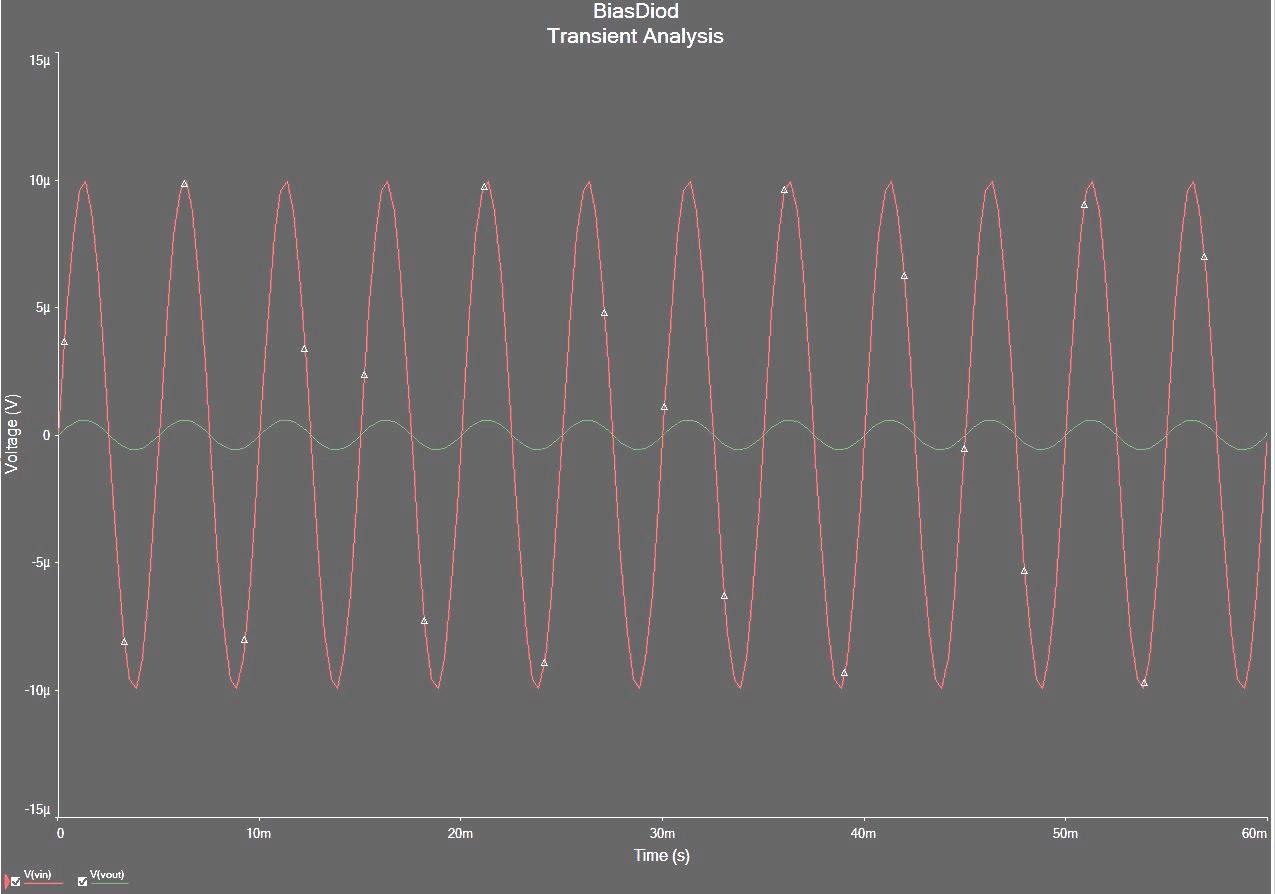
\includegraphics[width=0.5\textwidth]{figure/1}
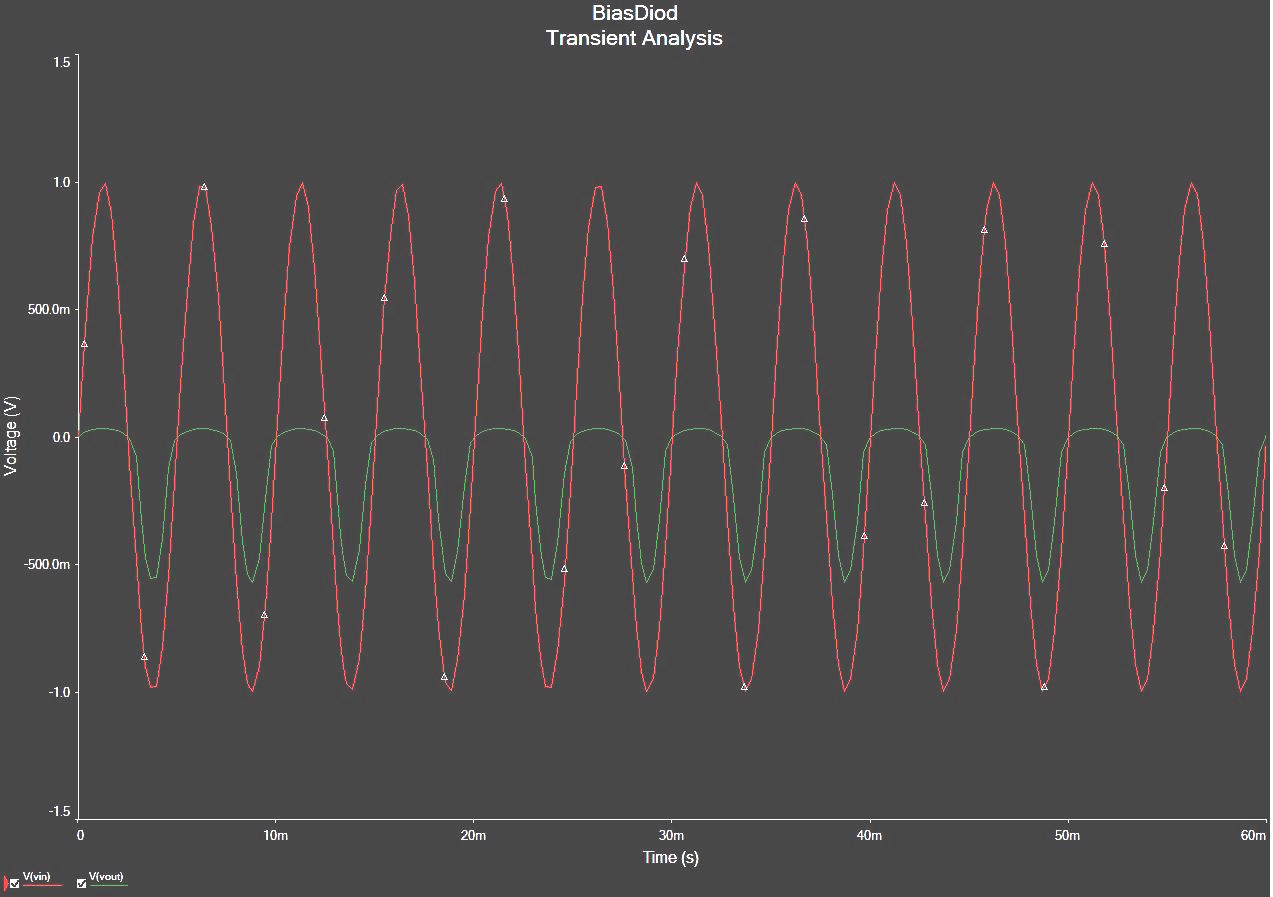
\includegraphics[width=0.5\textwidth]{figure/Part2-Part1}
\caption{Input signal(red) and output signal(green). Top: At amplitude =$1\times10^{-5}$V. Bottom: At amplitude =1V}
\label{firstrow}
\end{figure}
\par  We use the Fourier decomposition to determine the purity of the waves. The Fourier analysis of the output and input signals are shown below. As shown in Fig.\ref{fourier1} he strength of the second harmonic of the output signal is 8 orders of magnitude stronger than that of the input. 
\begin{figure}[h!]
\center
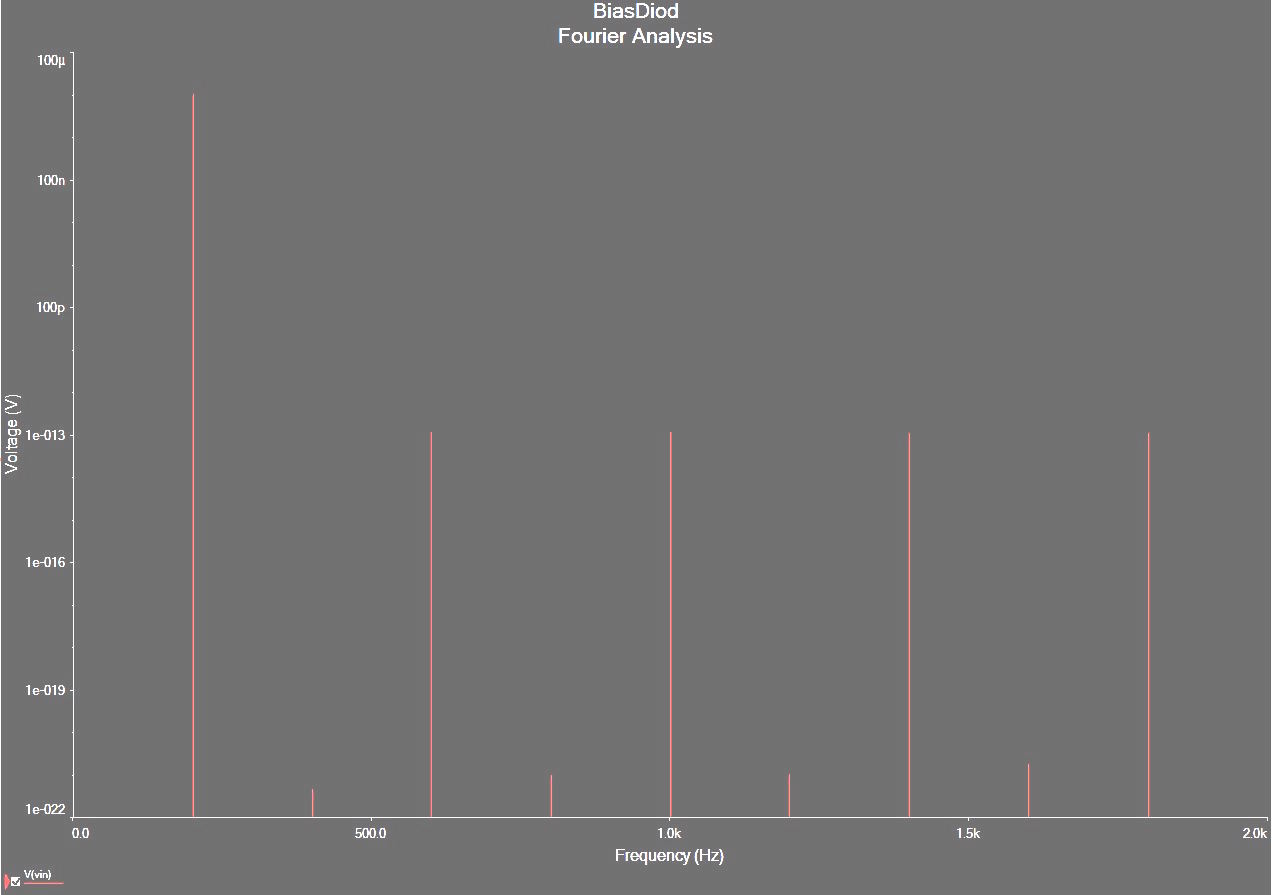
\includegraphics[width=0.5\textwidth]{figure/V_in_2}
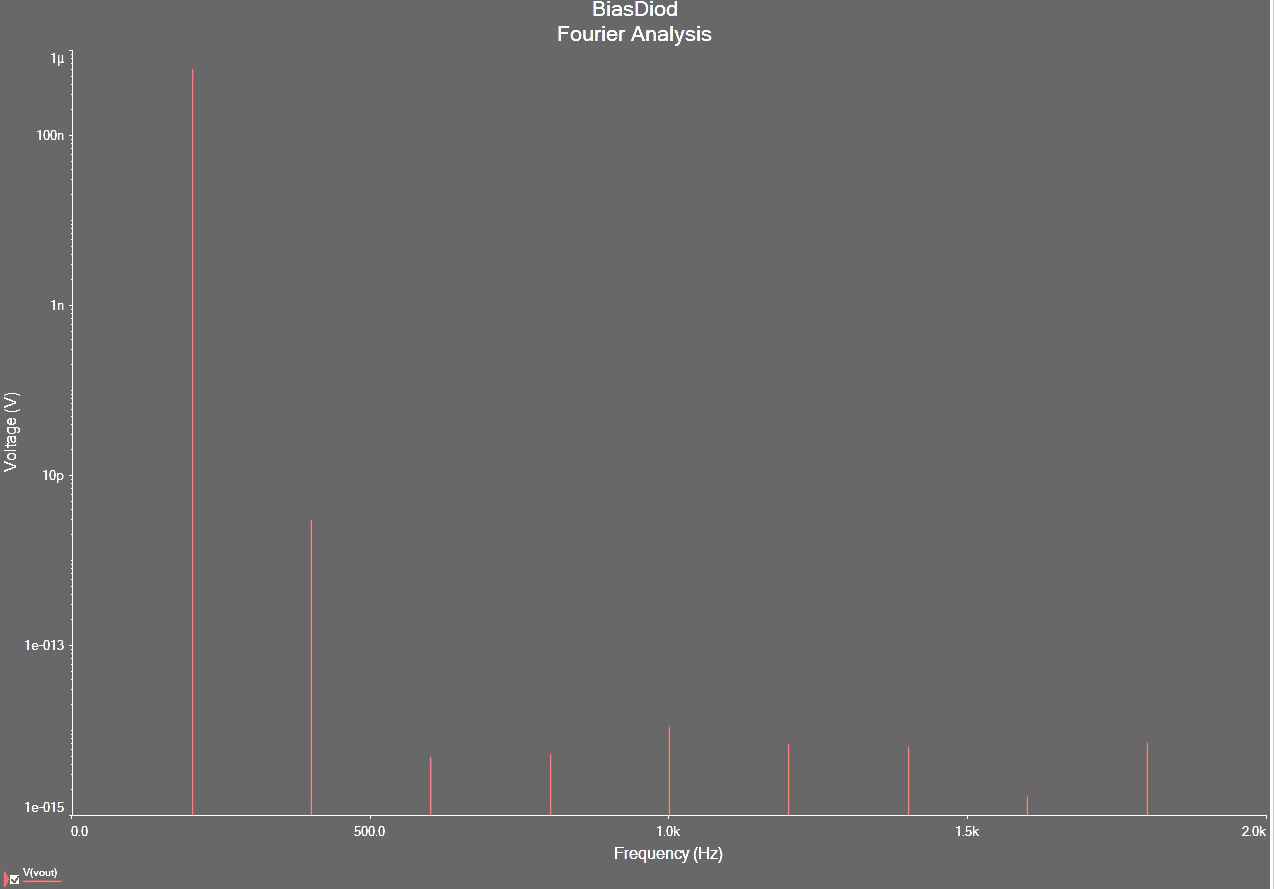
\includegraphics[width=0.5\textwidth]{figure/V_out_2}
\caption{ Top: Input signal. Bottom: Output signal}
\label{fourier1}
\end{figure}
\par We also examine the fourier decomposition of the output and input signal in Fig.\ref{fourier2}. Notice that the  positive component of the output signal has been rectified and flattened. As the signal has been cut-off in reverse bias, the flattening is due to the discharging of the capacitor, C1.  
\begin{figure}[h!]
\center
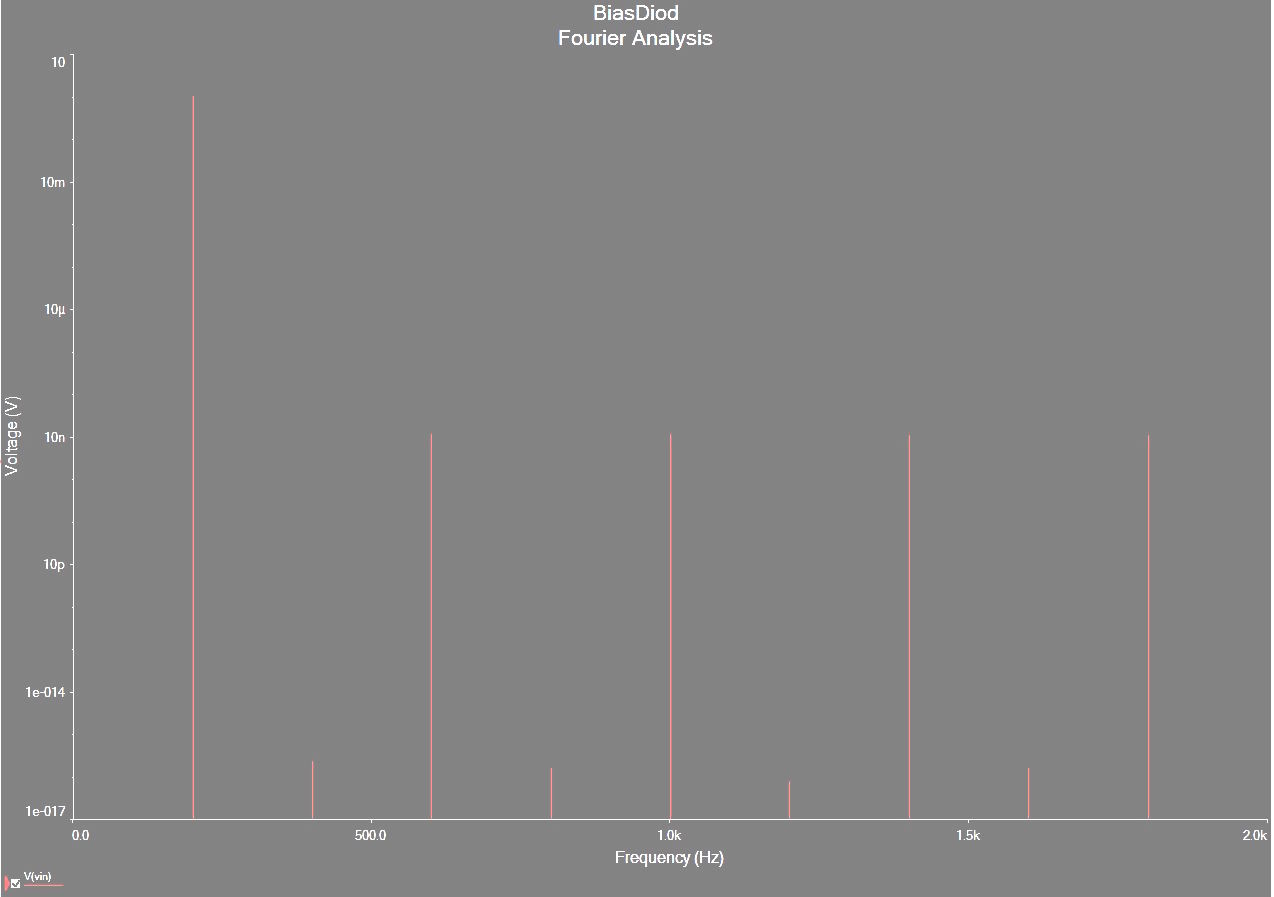
\includegraphics[width=0.5\textwidth]{figure/V_in_Part3or2}
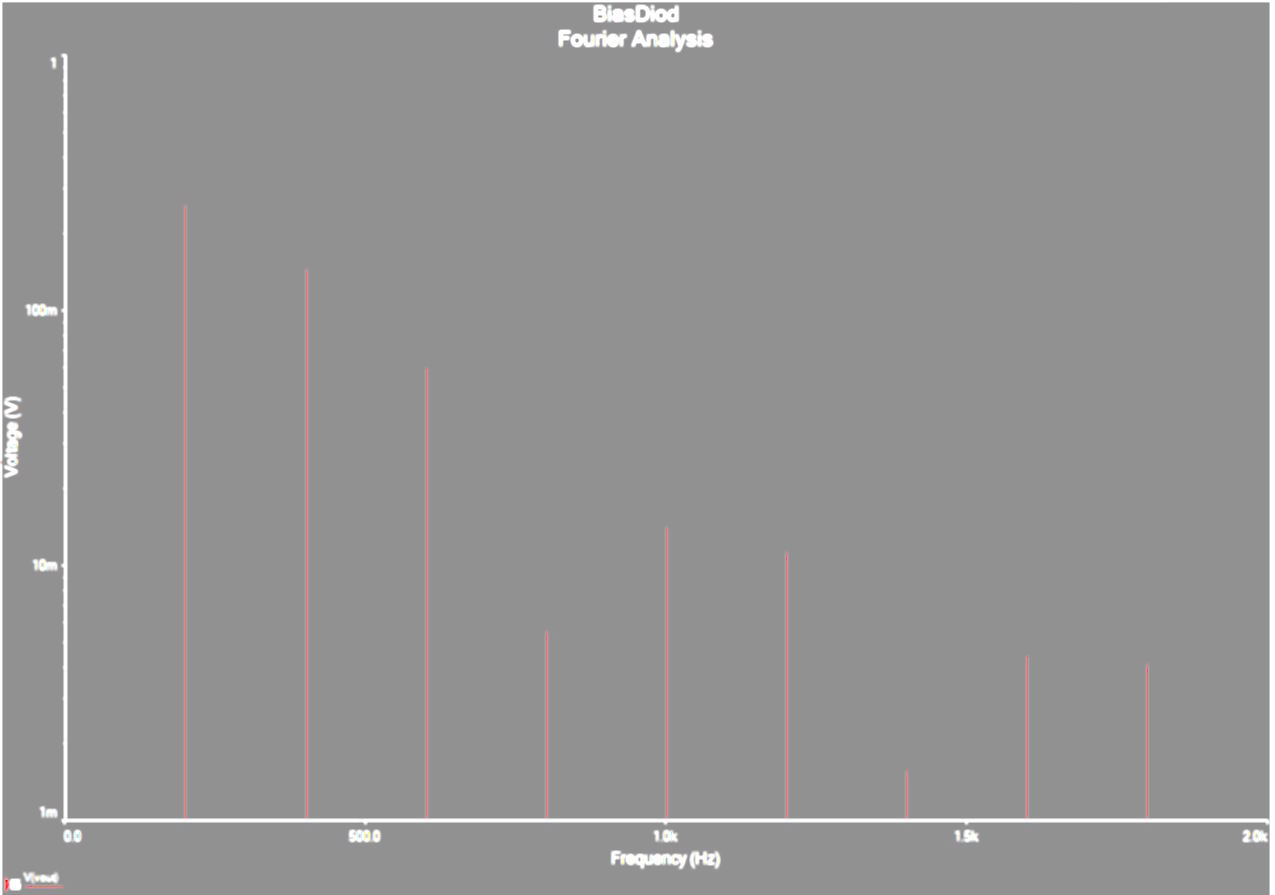
\includegraphics[width=0.5\textwidth]{figure/V_out_Part3actually2}
\caption{Top: Input signal. Bottom: Output signal}
\label{fourier2}
\end{figure}
\par Even though we see strong odd harmonics in the input signal, the output signa's harmonics is decreasing. The second harmonic is 15 orders of magnitude stronger in the output signal compared to the input signal and is only 1 order of magnitude lesser than the fundamental harmonic. There was no amplitude for which the second harmonic was stronger than the fundamental. The output signals for different values of the VAC are displayed below. The minimum order of magnitude where observe significant frequency doubling is at $10^{-5}$V. The second harmonic attenuates significantly from $10^{-5}$V to an order of magnitude lower as shown in the bottom most figure.
\begin{figure}
\center
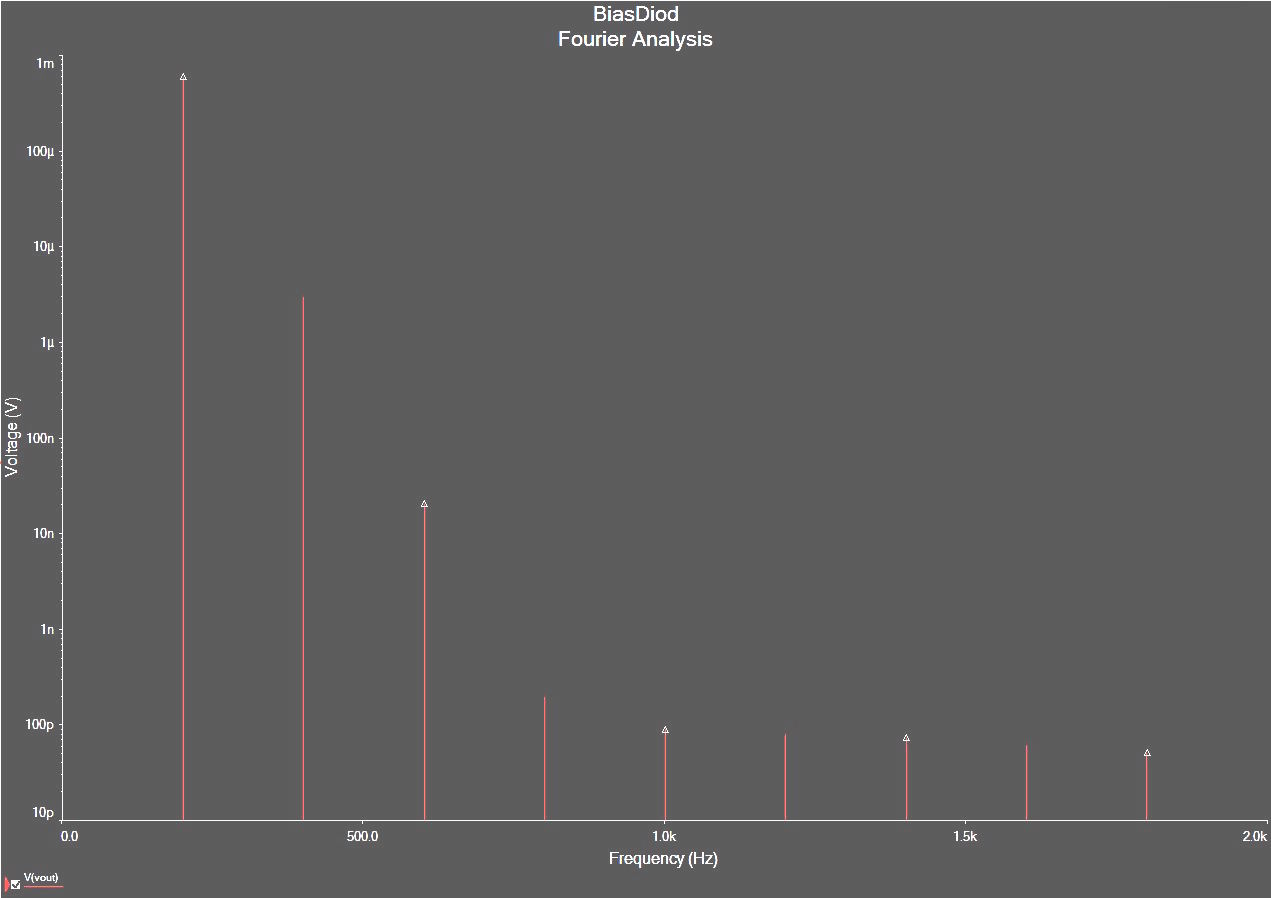
\includegraphics[width=0.5\textwidth]{figure/0_01V}
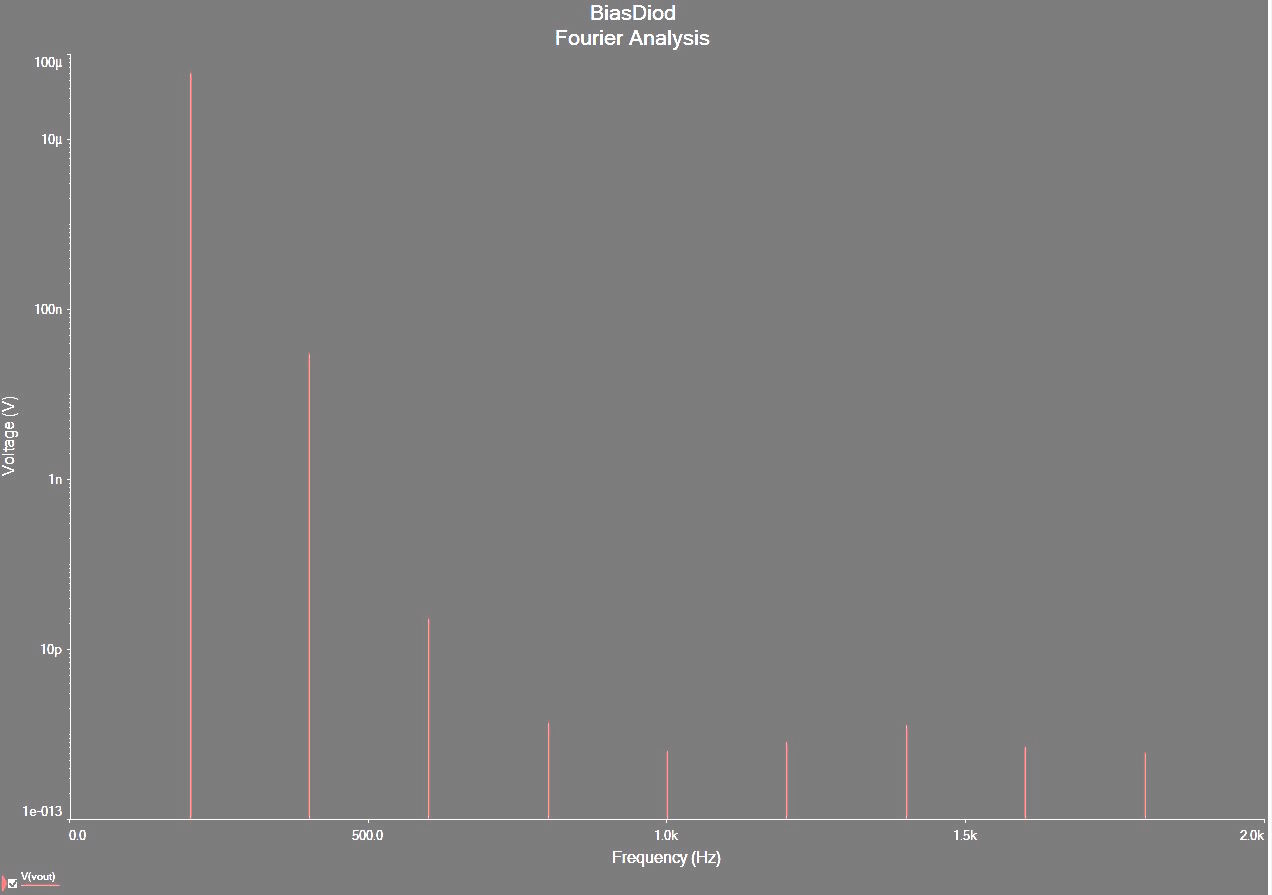
\includegraphics[width=0.5\textwidth]{figure/0_001V}
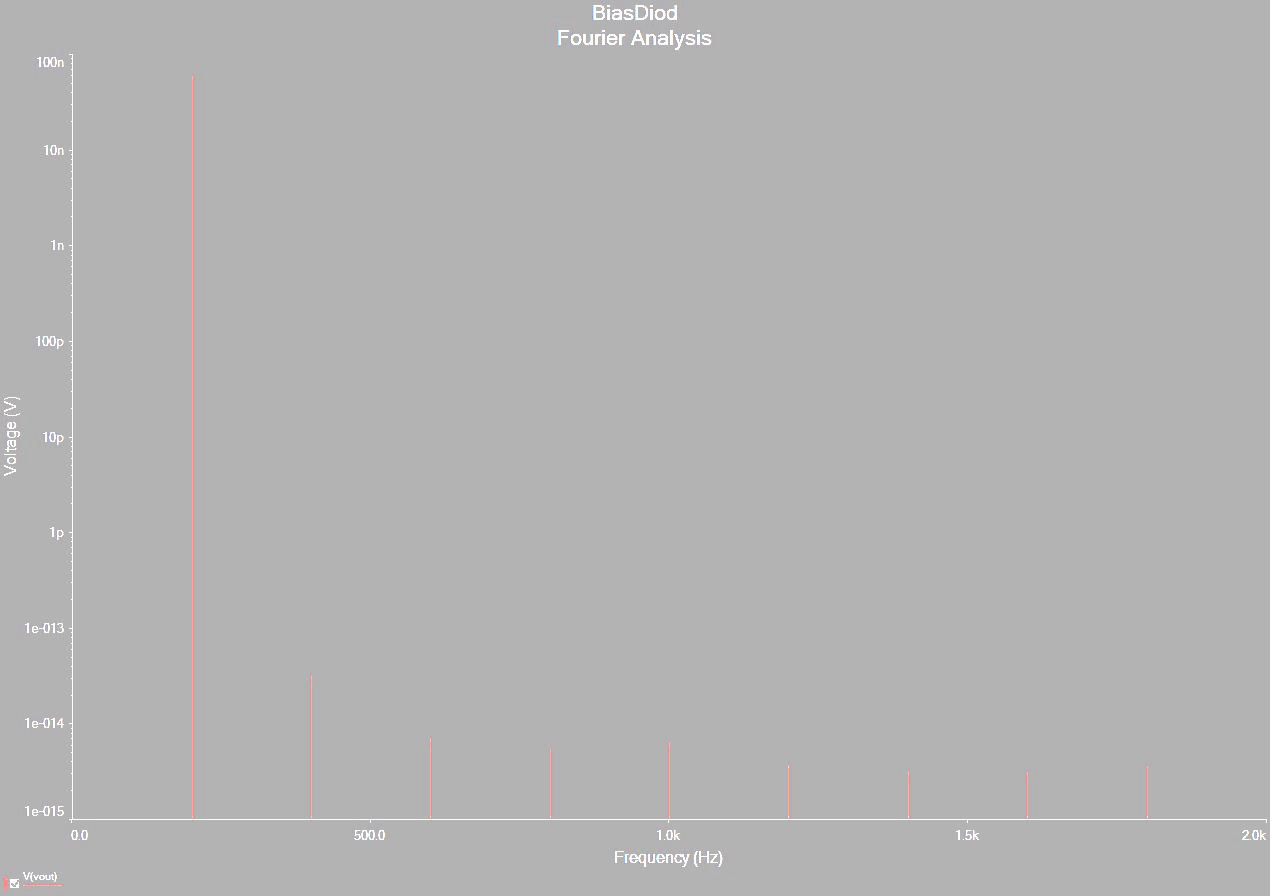
\includegraphics[width=0.5\textwidth]{figure/0_000001V}
\caption{Top: 0.01V. Middle:0.001V Bottom: 0.000001V}
\label{fourier3}
\end{figure}
\par  Frequency doubling is a phenomenon observed in non-linear circuits and is part of a broader response of frequency multiplying. When a pure sinusoidal wave is introduced into a non-linear circuit, it responds by distorting the signal and distributing the power across the higher harmonics. This is why we observe a significantly stronger second harmonic in the output signal.
\section*{Conclusion}
In this lab, we investigated the characteristics of semiconductor diodes . We explored the temperature-dependence of the diode using liquid nitrogen. Using CurveTracer and manually measuring the diode's voltage drop and current , we demonstrate the nonlinear VI relation of diodes. We further examine how a circuit behavior is altered with the addition of a diode and how their one-directional nature can be useful for various applications. We explore circuits that includes different types of diodes, such as light-emitting diode and zener diode, to investigate their characteristics and applications. 
%Diodes are useful --- their one directional characteristic
\section*{Acknowledgments}
\begin{footnotesize}
The author would like to acknowledge support from the GSI in this lab in addressing our questions about the lab and with the handling of liquid nitrogen. I would also like to thank my partner, Leah Tom, for helpful discussion and collaboration that helped this work. We also appreciate Sissi Wang for providing us with guidance on question 3.5, 3.8, and 3.9.
\end{footnotesize}
  \section*{References}
 \begin{footnotesize}
 \begin{itemize}
 \item Horowitz, Paul, and Winfield Hill. \textit{The Art of Electronics}. Cambridge: Cambridge UP, 1989. Print.
 \item ``Lab 3 - Diodes." \textit{Donald A. Glaser Advanced Lab.} Regents of the University of California, n.d. Web. 01 Feb. 2015.
  \item ``Zener Diode as Voltage Regulator Tutorial." Basic Electronics Tutorials. N.p., 13 Aug. 2013. Web. 14 Feb. 2015.
\end{itemize} 
  \end{footnotesize}

\end{document}
